\documentclass[10pt,a4paper]{article}
\usepackage[utf8]{inputenc}
\usepackage[ngerman]{babel}
\usepackage[left=2.5cm,right=2.5cm,top=4cm,bottom=3cm]{geometry} % Seitenränder 
\usepackage{amsmath}
\usepackage{amsfonts}
\usepackage{amssymb}
\usepackage{graphicx}
\usepackage{mathabx} % contains \Dashv
\usepackage{enumitem}
\usepackage{fancyhdr}

\title{Informatik der Syteme - Exercise 7}
\author{Jan Hoffmann, Mike Hengge}
\pagestyle{fancy}
% Header
\fancyhead[L]{\textbf{Informatik der Systeme}\\ \textbf{Exercise 6}}
\fancyhead[C]{}
\fancyhead[R]{Jan Hoffmann, Matr. 3177642\\ Mike Hengge, Matr. 3940400}
% Footer
\fancyfoot[L]{}
\fancyfoot[C]{}
\fancyfoot[R]{\thepage}

\begin{document}
\section*{Problem 7.2:}

	
\section*{Problem 7.3:}
	\item Es werden 4 Funktionsaufrufe benötigt um auf das 4. Fibonacci-Element zu kommen. \\\\\\
	\begin{minipage}[t]{0.4\linewidth}				
						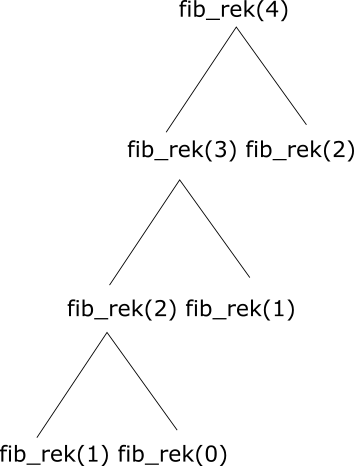
\includegraphics[scale=0.25]{baumstruktur.png}
					\end{minipage}	
\section*{Problem 7.4:}

\end{document}